%% Package and Class "uiucthesis2014" for use with LaTeX2e.
\documentclass[edeposit,fullpage]{uiucthesis2018}


\usepackage[acronym,toc]{glossaries}
\newacronym{crpg}{CRPG}{Computational Reactor Physics Group}
\newacronym{ornl}{ORNL}{Oak Ridge National Laboratory}
\newacronym{lanl}{LANL}{Los Alamos National Laboratory}
\newacronym{inl}{INL}{Idaho National Laboratory}
\newacronym{mit}{MIT}{Massachusets Institute of Technology}
\newacronym{csg}{CSG}{constructive solid geometry}
\newacronym{cfd}{CFD}{computational fluid dynamics}
\newacronym{cad}{CAD}{computer aided design}
\newacronym{dnp}{DNP}{delayed neutron precursor}
\newacronym{ghg}{GHG}{greenhouse gas}
\newacronym{gif}{GIF}{Generation IV International Forum}
\newacronym{msr}{MSR}{molten salt reactor}
\newacronym{msre}{MSRE}{Molten Salt Reactor Experiment}
\newacronym{msbr}{MSBR}{Molten Salt Breeder Reactor}
\newacronym{msfr}{MSFR}{Molten Sodium Fast Reactor}
\newacronym{nrc}{NRC}{Nuclear Regulatory Commission}
\newacronym{rnd}{R\&D}{research and development}
\newacronym{mns}{M\&S}{modeling and simulation}
\newacronym{ent}{E\&T}{education and training}
\newacronym{doene}{DOE-NE}{Department of Energy Office of Nuclear Energy}
\newacronym{cc}{CC}{closed code}
\newacronym{oss}{OSS}{open source software}
\newacronym{iaea}{IAEA}{International Atomic Energy Agency}
\newacronym{oncore}{ONCORE}{Open-source Nuclear COdes for REactor analysis}
\newacronym{snf}{SNF}{spent nuclear fuel}
\newacronym{sfr}{SFR}{sodium-cooled fast reactor}
\newacronym{doe}{DOE}{Department of Energy}
\newacronym{bol}{BOL}{beginning of life}
\newacronym{eol}{EOL}{end of life}
\newacronym{oop}{OOP}{object oriented programming}
\newacronym{tap}{TAP}{Transatomic Power}


\usepackage{xspace}
\usepackage{graphics}

\newcommand{\Cycamore}{\textsc{Cycamore}\xspace}
\newcommand{\Cyclus}{\textsc{Cyclus}\xspace}
\newcommand{\SaltProc}{\textsc{SaltProc}\xspace}
\newcommand{\OpenMC}{\textsc{OpenMC}\xspace}
\newcommand{\SerpentTWO}{\textsc{Serpent2}\xspace}
\newcommand{\ONIX}{\textsc{ONIX}\xspace}
\newcommand{\NJOYTWOONE}{\textsc{NJOY21}\xspace}
\newcommand{\ChemTriton}{\textsc{ChemTriton}\xspace}
\newcommand{\SCALE}{\textsc{SCALE}\xspace}
\newcommand{\TRITON}{\textsc{TRITON}\xspace}

\usepackage{placeins}
\usepackage{booktabs} % nice rules (thick lines) for tables
\usepackage{microtype} % improves typography for PDF

\usepackage[hyphens]{url}
\usepackage{hyperref}
\usepackage{subfig}
\usepackage{hhline}
\usepackage{amsmath}
\usepackage{color}
\usepackage{multirow}
\usepackage{siunitx} % typesetting for units
\sisetup{
    input-decimal-markers = .,input-ignore = {,},table-number-alignment = right,
    group-separator={,}, group-four-digits = true
}
\usepackage{booktabs}
\newcommand\tab[1][1cm]{\hspace*{#1}}

\usepackage{threeparttable, tablefootnote}

%tikzpicture fit to page width
\usepackage{environ}
\makeatletter
\newsavebox{\measure@tikzpicture}
\NewEnviron{scaletikzpicturetowidth}[1]{%
  \def\tikz@width{#1}%
  \def\tikzscale{1}\begin{lrbox}{\measure@tikzpicture}%
  \BODY
  \end{lrbox}
  \pgfmathparse{#1/\wd\measure@tikzpicture}%
  \edef\tikzscale{\pgfmathresult}%
  \BODY
}

\usepackage{tabularx}
\newcolumntype{b}{>{\hsize=1.0\hsize}X}
\newcolumntype{q}{>{\hsize=0.5\hsize}X}
\newcolumntype{R}{>{\raggedleft\arraybackslash\hsize=0.5\hsize}X}
\newcolumntype{z}{>{\hsize=0.75\hsize}X}
\newcolumntype{s}{>{\hsize=.5\hsize}X}
\newcolumntype{m}{>{\hsize=.75\hsize}X}

\usepackage{cleveref}
\usepackage{datatool}
\usepackage[numbers]{natbib}
\usepackage{notoccite}


\usepackage{tikz}
\usetikzlibrary{positioning, arrows, decorations, shapes}

\usetikzlibrary{shapes.geometric,arrows}
\tikzstyle{process} = [rectangle, rounded corners, minimum width=2.5cm, minimum height=1cm,text centered, draw=black, fill=blue!30]

\tikzstyle{object} = [ellipse, rounded corners, minimum width=3cm, minimum height=1cm,text centered, draw=black, fill=green!30]
\tikzstyle{objectr} = [ellipse, rounded corners, minimum width=3cm, minimum height=1cm,text centered, draw=black, fill=red!30]

\tikzstyle{empty} =  [rectangle, rounded corners, minimum width=2.5cm, minimum height=0.7cm,text centered, draw=black, fill=white!30]
\tikzstyle{arrow} = [thick,->,>=stealth]


\title{Implementation and validation of \OpenMC in \SaltProc}
\author{Oleksandr Redin Yardas}
\department{Nuclear, Plasma, Radiological Engineering}
\schools{B.A., Grinnell College, 2020}
\msthesis
\advisor{Madicken Munk}
\degreeyear{2022}
\committee{Research Scientist Madicken Munk, Advisor \\ ... }


\begin{document}
\maketitle

\frontmatter
%% Create an abstract that can also be used for the ProQuest abstract.
%% Note that ProQuest truncates their abstracts at 350 words.
\begin{abstract}

Abstract.

\end{abstract}

\chapter*{Acknowledgments}

Acks.

%% The thesis format requires the Table of Contents to come
%% before any other major sections, all of these sections after
%% the Table of Contents must be listed therein (i.e., use \chapter,
%% not \chapter*).  Common sections to have between the Table of
%% Contents and the main text are:
%%
%% List of Tables
%% List of Figures
%% List Symbols and/or Abbreviations
%% etc.

\tableofcontents
\listoftables
\listoffigures

%% Create a List of Abbreviations. The left column
%% is 1 inch wide and left-justified
%\chapter{List of Abbreviations}
%\printglossaries
%% Create a List of Symbols. The left column
%% is 0.7 inch wide and centered

\pagebreak
\mainmatter

\chapter{Introduction}%
\label{cha:introduction}
%
%\section{Motivation}%
%\label{sec:motivation}
%
%Increasing \gls{ghg} emissions due to human activity since the Industrial
%Revolution drives observed increases in average global surface temperature via
%the greenhouse effect\cite{mitchell_greenhouse_1989}
%\cite{paola_a_arias_2021_ts} (\textbf{global warming}).  Observed impacts of
%global warming and associated phenomena include decreased yields in agriculture
%and aquaculture, increased prevalance and impacts of extreme climatic events,
%and overwhelmingly inequitable impacts on historically marginalized groups
%\cite{hans_portner_2022_ts}. Figures \ref{fig:ipcc-ts3-a} and
%\ref{fig:ipcc-ts3-b} summarize impacts on ecosystems and human systems,
%respectively. Notice the overwhelmingly negative impacts on health and infrastructure in human systems.
%
%\begin{figure}[htpb]
%    \centering
%    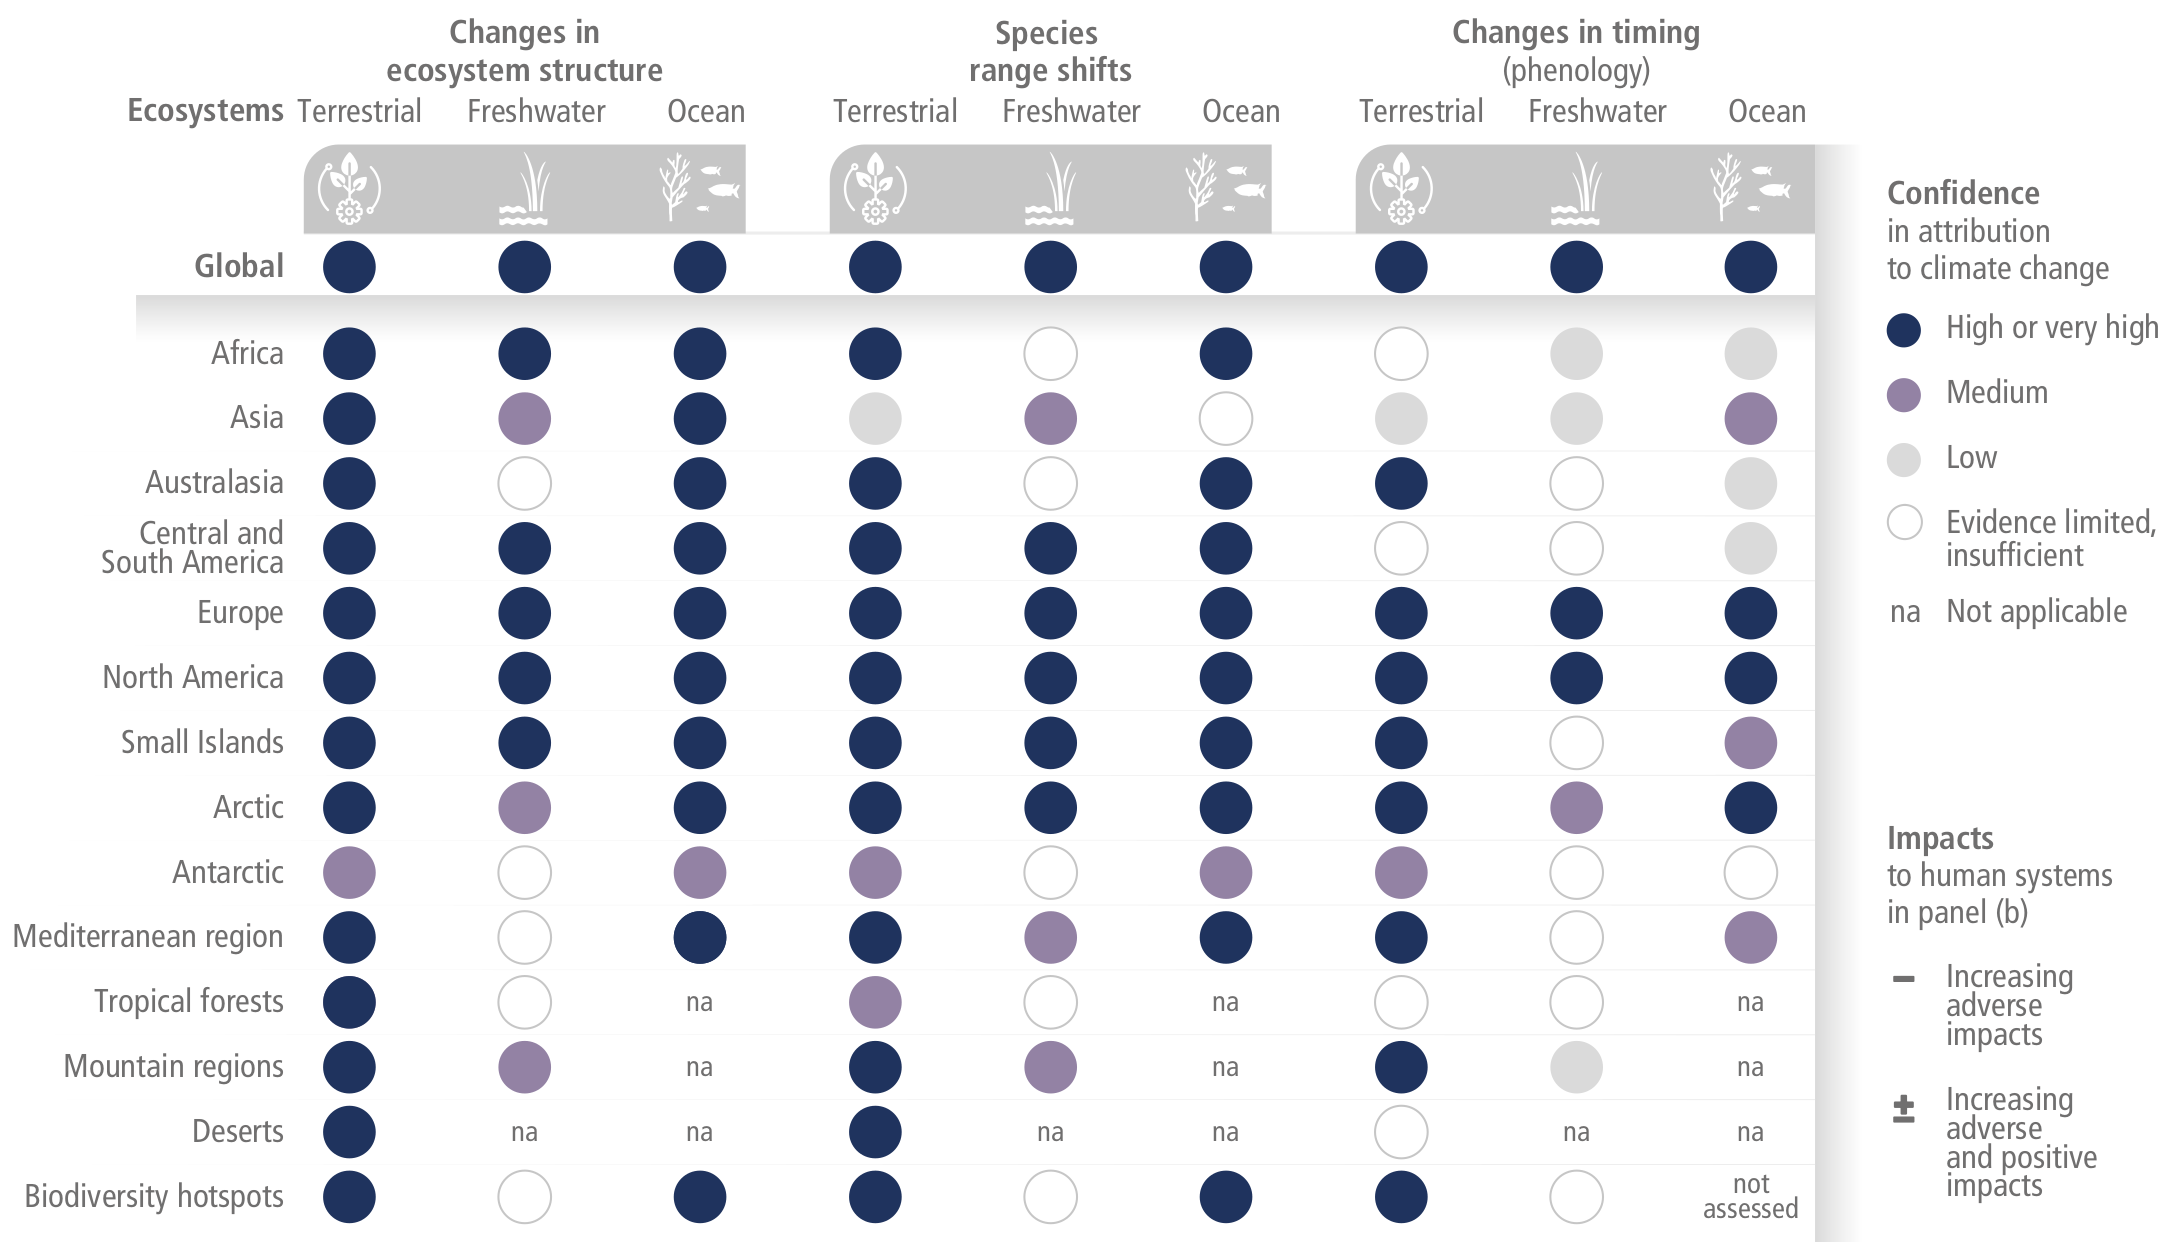
\includegraphics[width=0.8\textwidth]{figs/ipcc-ts3-a.png}
%    \caption{Observed impacts of climate change on ecosystems. From \cite{hans_portner_2022_ts}}
%    \label{fig:ipcc-ts3-a}
%\end{figure}
%
%\begin{figure}[htpb]
%    \centering
%    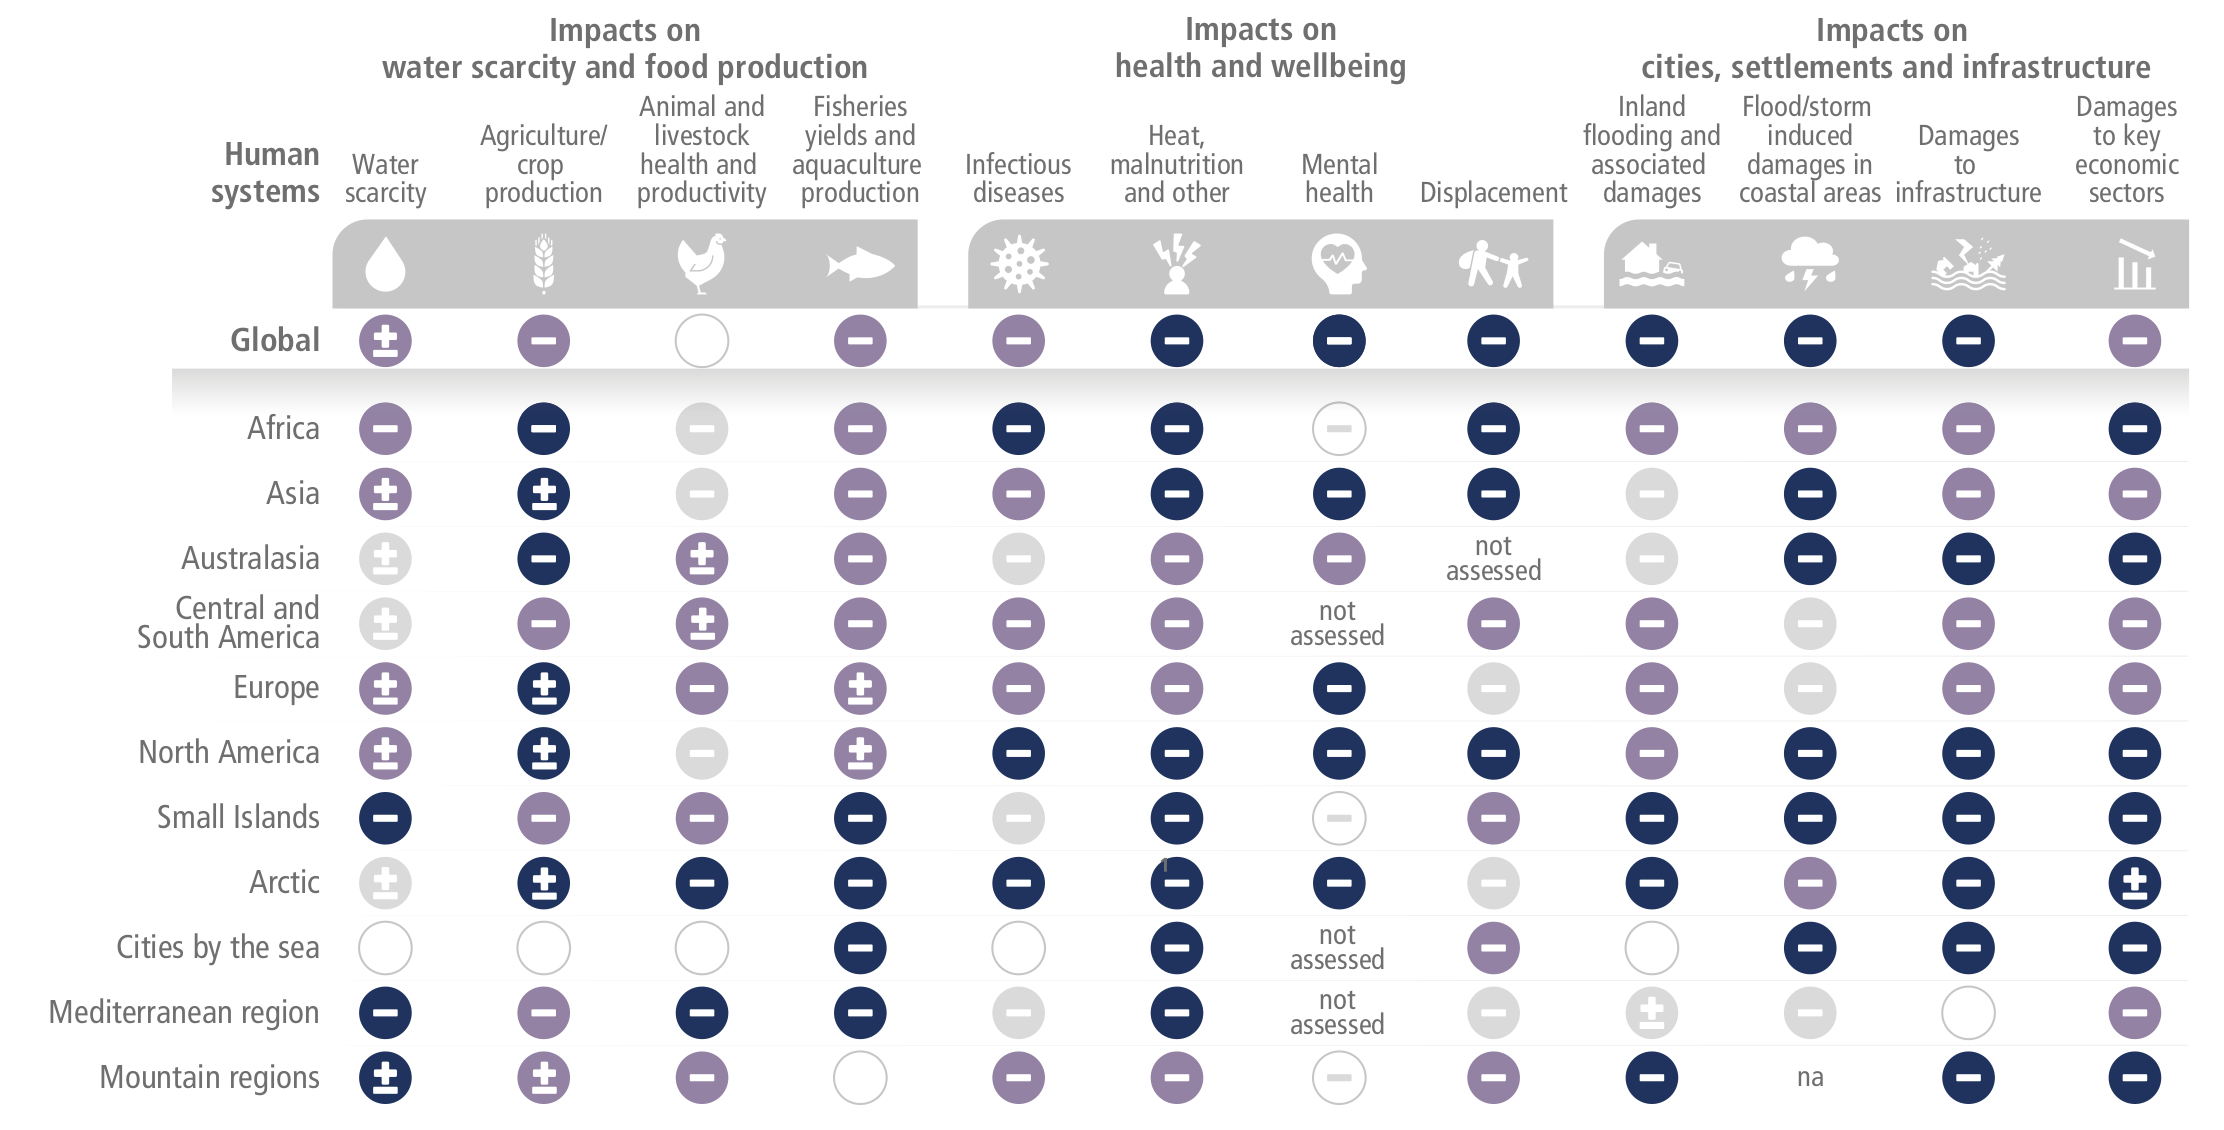
\includegraphics[width=0.8\textwidth]{figs/ipcc-ts3-b.png}
%    \caption{Observed impacts of climate change on human systems. From \cite{hans_portner_2022_ts}}
%    \label{fig:ipcc-ts3-b}
%\end{figure}
%
%Projected impacts of global warming include further ecosystem disruption and
%degradation, risks to global food security, and risks to general well being and
%livelihoods \cite{hans_portner_2022_ts}. Transitioning from fossil
%fuel-based electricity production methods to zero-emission
%\footnote{zero-emissions during operation; there are life-cycle carbon costs
%associated with any form of power production} electricity production methods
%(\textbf{decarbonization}) would contribute significantly to a global \Gls{ghg}
%emission reduction, and, in turn, dampen the effects of global
%warming\cite{minal_pathak_2022_ts}. Our three main options for decarbonization
%are renewables (such as solar, wind, and geothermal), hydropower, and nuclear power. We will
%need all of these technologies working together if we want to successfully
%decarbonize (cite). However, each technology has a specific use case where it works
%best. Solar and wind are best suited for storing up energy for later use on a
%large scale,\footnote{this is a product of the {\it intermittency} of wind and
%solar; solar intensity and wind speed are highly variable and unpredictable
%long term} which can then offset rapid fluctuations in electricity usage.
%Nuclear, hydropower, and geothermal are better suited to provide
%base-load power\cite{eia_electricity_2021}. Geothermal and hydropower are
%limited by geographical features (geothermal activity and elevated water
%sources), making nuclear the most flexible option\footnote{provided a suitable
%coolant exists. The majority of currently operating nuclear power plants are
%water-cooled and thus require a large water source such as a river, lake, or
%ocean.} for a future carbon-free base-load. Therefore, we should
%maintain and develop nuclear power technologies so they can contribute to
%decarbonization efforts.\footnote{despite these positive qualities, nuclear
%power is a divisive technology with legitimate technological and policy
%concerns. Fortunately, many of these concerns have technological and procedural
%solutions}
%
\section{Current and Future Trajectories of Nuclear Power}%
\label{sec:current_and_future_trajectories_of_nuclear_power}
Nuclear power currently constitutes one fifth of US domestic electricity
production and half of US zero-carbon electricity production
\cite{eia_faq_2021} \cite{doene_facts_2021}. The current US nuclear
fleet faces several threats to its future. The most relevant of
these is the state of the electricity market: record-low natural gas prices and
increases in subsidies for renewables without similar compensation for
nuclear make it uncompetitive in the current market and economically unsustainable in the
long term if current conditions continue\footnote{This is a generalization as
the economics of electricity markets is incredibly complex and requires more space that I can give to it
in this thesis to fully appreciate} \cite{szilard_economic_2016}.
%perhaps mention all plants that have been shut down recently?

Assuming that we resolve the economic threats to our current nuclear fleet, they
are -- like all things -- subject to aging and deterioration; at some point in
the future, we will need to shut down and decommission them. 
Nuclear power will be a key player in decarbonization
strategies used in the future. To maintain nuclear power's position in our decarbonization technology
stack, we will need to develop and implement new kinds of nuclear reactors that
are more sustainable, economically competitive, safe, and reliable than their
predecessors. There are several designs that are currently of interest for future
deployment considerations.
%% I want to make this point differently... the conclusion should be that we need new nuclear power tech to ensure we can decarbonize, but I don't feel like the preceding statements smoothly come to that conclusion in the way I have preseneted them here
 
%#\section{Molten Salt Reactors}%
%\label{sec:molten_salt_reactors}
%
%The first generation of nuclear power reactors includes the early prototypes and
%civil deployments in pursuit of cheap and bountiful energy. The second
%generation of reactors was built on top of this momentum, and most reactors
%operating today are from this generation. Following the well publicized and
%documented accidents at Three Mile Island (1976) and Chernobyl (1981) power
%plants, the third generation of nuclear power developed with increased safety
%and reactor lifetime in mind, however these reactors failed to replicate the
%relative success and widespread use of second generation reactors.
This new generation of nuclear power reactors will need to rapidly respond to increasing
electricity consumption and the need for decarbonization. These reactors need
to be built quickly and have widespread use, while maintaining or increasing
fuel efficiency, economic competitiveness, safety, and proliferation resistance.

This is the conclusion that the \Gls{gif} -- a ``co-operative
international endeavor seeking to develop the feasibility and performance of
fourth generation nuclear systems'' \cite{gif_homepage} -- came to in their 2002
roadmap \cite{doe-ne_technology_2002}. The \Gls{gif} selected six reactor
technologies in total. One of them, the \Gls{msr},\footnote{for
this thesis {\it Molten Salt Reactor} refers specifically to the reactor type
where the fissile material is dissolved in in the salt} is of
particular interest due to the unique opportunities and challenges it presents
for new nuclear fuel cycles, proliferation safeguards, and multiphysics
modeling.
%% why the msr??

The \Gls{msr} is so named as it is a nuclear reactor that uses a mixture of
liquid-phase salts as a coolant and solvent for the fuel. Liquid fuel enables
the adoption of {\it online reprocessing} by pumping used fuel out of the
reactor core and pumping fresh or reprocessed fuel back into the reactor core.
\footnote{this concept is known as {\it separations and feeds}} This
enables the removal of undesirable fission products -- neutron absorbers in
particular -- produced by the fission reaction. This also allows for better
utilization of fission neutrons in the fuel. In contrast, while solid-fueled
reactors will shuffle the fuel within the assembly over time, the fission
products remain trapped in the fuel. This can reduce the thermal performance of
the fuel via thermal cracking and absorb neutrons that would otherwise
contribute to the fission reaction. This also means that fuel will be burned
unevenly unless carefully managed

\Gls{msr}s face several technical and logistical challenges before we can
deploy them for civilian power generation. High temperature liquid-phase salt
will steadily corrode metals over time, so the reactor vessel of a \Gls{msr}
must use special corrosion-resistant materials. High temperature salt itself is
extremely hazardous and reacts explosively with moisture, so workers handling
fuel salt must use special procedures and PPE. Remote handling of fuel salt may
be necessary for certain tasks. Even with such challenges, the 
potential benefits of \Gls{msr} technology merit further investigation
into its development.

\Gls{mns} codes will play a critical role in licensing GenIV reactors. In
preparation for \Gls{msr} deployment, both the \Gls{doene} and the \Gls{nrc}
identified several technical gaps in current \Gls{mns} tools that are necessary
for license application reviews
\cite{betzler_modeling_2019} \cite{usnrc_nonlwr_2020-1}. In particular, both the
\Gls{doene} and the \Gls{nrc} have identified fuel composition and its
evolution in \Gls{msr}s to be key modeling features necessary for accident
analysis. 

\section{\Gls{msr} Depletion Codes}%
\label{sec:msr_codes}

To model the changing fuel composition in a \Gls{msr}, there are at least two
processes we must consider:
\begin{enumerate}
    \item Fuel {\it depletion}\footnote{the consumption of fissile material in the fuel and production of fission products via the fission chain reaction} driven my the migration and absorption of neutrons and fuel in the core.
    \item Removal and feed processes of fission products and fuel, respectively.
\end{enumerate}

The Bateman equation describes the process of depletion for any nuclide $i$, or
mathematically, the rate of change of the number density of a nuclide in a nuclear reaction:

\begin{align}
    \label{eq:bateman-1}
    \frac{dN_{i}}{dt} =& \sum_{j} l_{j\to i}\lambda_{j} N_{j} + \gamma_{i} \Sigma^{f}_{j}\phi + \phi N_{i-1} \sigma^{a}_{i-1} - \lambda_{i}N_{i} - N_{i}\sigma^{a}_{i}\phi\\
    \text{where} & \nonumber \\
    N_{x} =& \text{number density for nuclide $x$ $[cm^{-3}]$}\nonumber\\
    l_{j\to i} =& \text{branching ratio for decay mode of nuclide $j$ that produces nuclide $i$ $[-]$}\nonumber\\
    \lambda_{x} =& \text{decay constant of nuclide $x$ $[s^{-1}]$}\nonumber\\
    \gamma_{i} =& \text{fission yield fraction for nuclide $i$ $[-]$}\nonumber \\
    \Sigma^{f}_{j} =& \text{average macroscopic fission cross section for nuclide $j$ $[cm^{-1}]$}\nonumber\\
    \phi =& \text{neutron flux $[cm^{-2}s^{-1}]$}\nonumber\\
    \sigma^{a}_{x} =& \text{neutron absorption cross-section for nuclide $x$ $[cm^{-2}]$}\nonumber\\
\end{align}
    
When solving for $n$ nuclides, we solve the matrix problem
$\frac{d}{dt}N(t) = \mathbf{A}N(t)$, where $N$ is an $n$-vector and
$\mathbf{A}$ contains all the coefficient terms in equation \ref{eq:bateman-1}.
Incorporating removals and feeds into equation \ref{eq:bateman-1} involves the
addition of a time dependent removal factor $r_{i}(t)$ and feed factor
$f_{i}(t)$. The resulting equation describes {\it continuous reprocessing}.
For $n$ nuclides, the matrix problem is then
$\frac{d}{dt}N(t) = \mathbf{A}N(t) + S(t)$, where $S$ is an $n$-vector
containing the sums of the removal and feed terms for each nuclide $i$. The
additional term in the Bateman equation from continuous reprocessing increases
computational cost and implementation difficulty and may require a different
set of preconditioners for numerical stability and convergence.

Alternatively, one could run a depletion simulation, perform the removals and
feeds in an external application on the resulting material composition, and run
another depletion simulation on the reprocessed composition. This procedure
models {\it batch-wise reprocessing}, in which material from the core is
reprocessed at regular intervals rather than continuously. Batch-wise
reprocessing enables flexibility in the choice of depletion solver, as an
external software tool can perform the reprocessing step and feed the results
back into the depletion solver.\footnote{this kind of coupling comes with its
own challenges, which are beyond the scope of this thesis}

\SaltProc\cite{rykhlevskii_saltproc_2018}, the focus of this thesis, uses a
batch-wise reprocessing approach to model the fuel composition in an \Gls{msr}
and uses \SerpentTWO\cite{leppanen_serpent_2014} to run depletion simulations.
\SaltProc is unique among its peers as an open source project\footnote{There are
other software projects that model fuel composition in \Gls{msr}s. Notably,
\ChemTriton\cite{betzler_molten_2017} -- a python script for \SCALE/\TRITON --
is functionally similar to \SaltProc. Section 1.2 in
\cite{rykhlevskii_fuel_2020} and section 4.2 in \cite{rykhlevskii_advanced_2018}
provide a high-level summary of other recent efforts}.

Historically, software used in licensing, \gls{rnd}, and \gls{ent} efforts in
the nuclear field have been closed source and proprietary. For \Gls{rnd} and
\Gls{ent} efforts in particular, the licensing process can bring collaborative
efforts to a grinding halt. Using \gls{cc}s in scientific publications and
research presents barriers to reproducibility and the ability of external
verification of results.
    
Regulatory bodies will require new software features (and, in some cases,
entirely new software tools) to effectively and efficiently perform licensing
activities for the next generation of advanced reactor designs
\cite{usnrc_nonlwr_2020-1}. Many of the open source tools emerging in the
past decade (e.g., \OpenMC\cite{romano_openmc_2015}) have the advantage over
their legacy \Gls{cc} ancestors (e.g., \SerpentTWO \cite{leppanen_serpent_2014})
of using best-practices for software development. Thus, the features
and tools required may be more readily implementable and usable in open source
projects than in closed codes.
    
We are entering the era of \gls{oss} purpose-built for nuclear
science and engineering applications. The number of open source projects in this
field
(\ONIX\cite{de_troullioud_de_lanversin_onix_2021}, \OpenMC,
\NJOYTWOONE\cite{noauthor_njoy21_2022}, \Cyclus\cite{noauthor_cyclus_2022}, to
name a few\footnote{the awesome-nuclear repository on GitHub
\cite{romano_awesome_2022} has good list of nuclear-related open source software
projects.}) is growing in recognition of the need for distributable,
high-quality, and transparent software tools. The
\Gls{iaea} facilitated \Gls{oncore} initiative \cite{fiorina_initiative_2021} is the best
example of the push towards \Gls{oss}, as seen in the mission
statement: to
``[promote] development and application of open-source multi-physics simulation
tools to support research, education, and training for analysis of advanced
nuclear power reactors'' \cite{iaea_open-source_2022}. 


\section{Objectives}%
\label{sec:objectives}

While \SaltProc itself is open source, \SerpentTWO is not. \OpenMC recently
added a \verb.deplete. module for fuel depletion simulations, meaning it is now
possible to have a fully open-source stack of dependencies for \SaltProc.
In this spirit, I have added support for \OpenMC to \SaltProc. \OpenMC support improves
the accessibility and usability of \SaltProc, and I hope that researchers
interested in \Gls{msr}s begin using and contributing to the tool.

This Master's thesis has two primary objectives
\begin{enumerate}
    \item Refactor \SaltProc to enable \OpenMC support, as well as enable
        easier implementation for other monte-carlo depletion codes in the
        future. 
    \item Verify the implementation on a \Gls{csg} model of the \Gls{msbr}\footnote{See
        Chapters 2 and 4 for a discussion of this choice.}
\end{enumerate}

It is my hope that with the addition of \OpenMC support, \SaltProc can have a
lower barrier-of-entry for researchers and students. 

The structure of this thesis is as follows:
\begin{itemize}
    \item Chapter \ref{ch:chapter2} describes the structure of \SaltProc and process of
        implementing support for \OpenMC in the context of past and current
        \Gls{msr} modeling efforts.
    \item Chapter \ref{ch:chapter3} describes the updated code structure and restates the
        formal mathematical representation of the reprocessing used in the
        SaltProc.
    \item Chapter \ref{ch:chapter4} describes the reactor design for verification purposes and
        specifies the inputs and settings.
    \item Chapter \ref{ch:chapter5} presents the results of the verification study and
        discusses their implications.
    \item Chapter \ref{ch:chapter6} summarizes the results, their implications, and suggests
        avenues for future work.
\end{itemize}


\chapter{Software Overview and Development}%
\label{cha:software_development}

A major component of this work was restructuring of the SaltProc code and implementation of OpenMC.
\section{SaltProc}%
\label{sec:saltproc}

SaltProc\cite{rykhlevskii_saltproc_2018} is an open source Python package that simulates on-line reprocessing via a batch-wise approach\footnote{Material is moved to or from the core at specific time intervals} in liquid-fueled \Gls{msr}s. More precisely, SaltProc manages material flows and separation processes on nuclides in the fuel. SaltProc relies on external codes to simulate fuel depletion.

The first version of SaltProc (v0.1) was a simple Python 2.7 package that used SERPENT 2 for the fuel depletion simulations. A single Python file contained all functions; separation processes applie dto  used an implicit 100\% efficiency \cite{rykhlevskii_advanced_2018}. The structure of SaltProc v0.1 did not lend itsef easily to development of more sophisticated treatments of reprocessing. This led to the release of Saltproc v0.2, in which the entire codebase was refactored into an object oriented
context in Python 3. The addition of new functionality in the \verb.Separator. and \verb.Process. classes enabled more sophisticated treatment of online reprocessing \cite{rykhlevskii_fuel_2020} 

SaltProc v0.3 saw the addition of gas sparging and ...

\section{OpenMC}%
\label{sec:openmc}

OpenMC \cite{romano_openmc_2015} is an open source Monte Carlo particle transport code. The \Gls{crpg} at \Gls{mit} started developing OpenMC back in 2011 with a focus on scalability for exascale computing. Since that time, developers new and old contributed features (cite?) and fixes to the tool expanding its scope and use cases. Notable features of OpenMC (as of version 0.12.1) are as follows \cite{openmc_homepage}:
\begin{itemize}
    \item Support for fixed source, $k$-eigenvalue, and subcritical neutron multiplication cacluclations.
    \item Support for \Gls{csg} and \Gls{cad} geometry.
    \item Support for both continuous and multigroup transport calculations.
    \item Support for parallel execution via MPI and OpenMP.
    \item Geometry visualization through the Python API.
\end{itemize}
The tool is now quite mature and feature-rich, rivaling its closed-source export controlled counterparts. 


Recently, depletion and photon transport were added by (who?)... The new depletion feature enables us to couple OpenMC to SaltProc and a fully open-source stack.

%\input{chapter3_methods}
%\input{chapter4_results}
%\input{chatper5_conclusions}

\chapter*{Appendix}
\appendix
\chapter*{Appendix B: SaltProc input file structure}
\label{appex:input-files}
\definecolor{bg}{rgb}{0.95,0.95,0.95}

\begin{listing}[!ht]
    \begin{minted}[frame=single,
                   framesep=3mm,
                   tabsize=4,
                   bgcolor=bg,
                   fontsize=\footnotesize]{json}
    {
      "Path to Serpent executable": "sss2",
      "File containing processing system objects": "msbr_objects.json",
      "Graph file containing processing system structure": "msbr.dot",
      "User's Serpent input file with reactor model": "msbr.serpent",
      "Path output data storing folder": "../../saltproc/data/",
      "Output HDF5 database file name": "msbr_kl_100_saltproc.h5",
      "Number of neutrons per generation": 50,
      "Number of active generations": 20,
      "Number of inactive generations": 20,
      "Restart simulation from the step when it stopped?": false,
      "Geometry file/files to use in Serpent runs": "geometry/msbr_full.ini",
      "Switch to another geometry when keff drops below 1?": false,
      "Salt mass flow rate throughout reactor core (g/s)": 9920000,
      "Number of steps for constant power and depletion interval case": 12,
      "Depletion step interval or Cumulative time (end of step) (d)": 3,
      "Reactor power or power step list during depletion step (W)": 2250000000
    }
    \end{minted}
    \caption{\SaltProc v0.3.0 input file}
    \label{listing:1}
\end{listing}

\begin{listing}[!ht]
    \begin{minted}[frame=single,
                   framesep=3mm,
                   tabsize=4,
                   bgcolor=bg,
                   fontsize=\footnotesize]{json}
    {
       "proc_input_file": "msbr_objects.json",
       "dot_input_file": "msbr.dot",
       "output_path": "./data",
       "num_depsteps": 12,
       "depcode": {
           "codename": "serpent",
           "exec_path": "sss2",
           "template_inputfile_path": "./msbr.serpent",
           "iter_inputfile": "saltproc_serpent",
           "iter_matfile": "saltproc_mat",
           "npop": 50,
           "active_cycles": 20,
           "inactive_cycles": 20,
           "geo_file_paths": ["./geometry/msbr_full.ini"]
       },
       "simulation": {
           "sim_name": "msbr_example_simulation",
           "db_name": "msbr_kl_100_saltproc.h5",
           "restart_flag": false,
           "adjust_geo": false
       },
       "reactor": {
           "volume": 1.0,
           "mass_flowrate": 9920000,
           "power_levels": [ 2250000000 ],
           "dep_step_length_cumulative": [ 3 ]
       }
    }
    \end{minted}
    \caption{\SaltProc v0.4.0 input file}
    \label{listing:2}
\end{listing}

\begin{listing}[!ht]
    \begin{minted}[frame=single,
                   framesep=3mm,
                   tabsize=4,
                   bgcolor=bg,
                   fontsize=\footnotesize]{json}
    {
       "proc_input_file": "msbr_objects.json",
       "dot_input_file": "msbr.dot",
       "n_depletion_steps": 12,
       "depcode": {
           "codename": "serpent",
           "template_input_file_path": "msbr.serpent",
           "geo_file_paths": ["geometry/msbr_full.ini"]
       },
       "simulation": {
           "sim_name": "msbr_kl_100_simulation"
       },
       "reactor": {
           "volume": 1.0,
           "mass_flowrate": 9920000,
           "power_levels": [ 2250000000 ],
           "depletion_timesteps": [ 3 ],
           "timestep_units": "d"
       }
    }
    \end{minted}
    \caption{\SaltProc v0.5.0 input file}
    \label{listing:3}
\end{listing}




\backmatter

\bibliographystyle{apalike}
\bibliography{bibliography}

\end{document}
\endinput
%%
%% End of file `thesis-ex.tex'.
